\documentclass[portrait,final,a0paper,fontscale=0.30]{baposter}
\setlength{\leftmargini}{1em}
%% read in constants, custom functions and used packages

%%%%%%%%%%%%%%%%%%%%%%%%%%%%%%%%%%%%%%%%%%%%%%%%%%%%%%%%%%%%%%%%%%%%%%%% Lit 
\usepackage[backend=biber, 
			style=ieee,
			url=false, 
			doi=true]{biblatex}
			
\addbibresource{refs.bib} % References path
\AtBeginBibliography{\tiny} % font size for references
\setlength{\bibitemsep}{0.5pt}
%%%%%%%%%%%%%%%%%%%%%%%%%%%%%%%%%%%%%%%%%%%%%%%%%%%%%%%%%%%%%%%%%%%%%%%% Image 
\usepackage{graphicx}
\graphicspath{{logos/}{figures/}} % paths for images

%%%%%%%%%%%%%%%%%%%%%%%%%%%%%%%%%%%%%%%%%%%%%%%%%%%%%%%%%%%%%%%%%%%%%%%% Color Settings
\usepackage{xcolor}
\definecolor{iftucfont}{RGB}{74,130,70}
\definecolor{iftuccolor}{RGB}{143,168,92}
\definecolor{iftucbackground}{RGB}{241,244,234}

%%%%%%%%%%%%%%%%%%%%%%%%%%%%%%%%%%%%%%%%%%%%%%%%%%%%%%%%%%%%%%%%%%%%%%%% Font Settings
\usepackage[sfdefault, regular]{roboto}

%%%%%%%%%%%%%%%%%%%%%%%%%%%%%%%%%%%%%%%%%%%%%%%%%%%%%%%%%%%%%%%%%%%%%%%% Layout  Settings
%% Allow multicolumns
\usepackage{multicol}
\setlength{\columnsep}{1.5em}
\setlength{\columnseprule}{0mm}

%% Row Settings
\usepackage{setspace}% for \onehalfspacing
\usepackage{parskip}

%% Control layout of itemize, enumerate, description
\usepackage{enumitem}

% page borders and header height
\usepackage{geometry}
\geometry{
	left=35pt,
	right=5pt,
	top=10pt
}

\newcommand{\compresslist}{% Define a command to reduce spacing within itemize/enumerate environments, e.g. \begin{itemize}\compresslist
			\setlength{\itemsep}{1pt}
			\setlength{\parskip}{0pt}
			\setlength{\parsep}{0pt}
		}
	
\newcommand{\compressbib}{%
		\setlength{\itemsep}{0pt}
		\setlength{\parskip}{0pt}
		\setlength{\parsep}{0pt}}
	
%%%%%%%%%%%%%%%%%%%%%%%%%%%%%%%%%%%%%%%%%%%%%%%%%%%%%%%%%%%%%%%%%%%%%%%% Table and figure settings
\usepackage{float, booktabs,array}

% Adjust row width in tables 
\renewcommand{\arraystretch}{1.2}

% for awesome plots and tables from files like .csv
\usepackage{pgfplots}\pgfplotsset{compat=newest}
\usepackage{pgfplotstable}

% Graphics package-alike macros for “general” boxes. Like resizing figures and aligning minipages
\usepackage{adjustbox}

% Add captions to your table or figure
\usepackage[
font=small,
labelfont=bf,
%labelfont=sc, %Kapitälchen, passt nicht wg. nicht-osf Ziffern
%%%%labelfont=it, %italics, 
%%%labelfont=sl, %slanted,
hypcap=true,
format=hang,
%margin={2cm,2cm}
width=0.8\linewidth
]{caption}

%%%%%%%%%%%%%%%%%%%%%%%%%%%%%%%%%%%%%%%%%%%%%%%%%%%%%%%%%%%%%%%%%%%%%%%% Other packages
% to help with long equations
\usepackage{amsmath}

% for todo notes
\usepackage{todonotes} 

% for comment blocks
\usepackage{verbatim}

% link URLs
\usepackage{url}

% dummy text 
\usepackage{lipsum}


\begin{document}

\begin{poster}%
	% Poster Options
	{
		% Show grid to help with alignment
		grid=false,
		% Number of columns and column spacing
		columns=6,
		colspacing=1em,
		% Color style
		bgColorOne=white,
		borderColor=iftuccolor,
		headerColorOne=iftucbackground,
		headerFontColor=iftucfont,
		boxColorOne=white,
		% Format of textbox
		textborder=rounded,
		textfont=\scriptsize,
		% Format of text header
		eyecatcher=true,
		headerborder=open,
		headerheight=0.1\textheight,
		%  textfont=\sc, An example of changing the text font
		headershape=rounded,
		headershade=plain,
		headerfont=\Large\bf, %Sans Serif
		% textfont={\setlength{\parindent}{1.5em}},
		boxshade=plain,
		%  background=shade-tb,
		background=plain,
		linewidth=1pt
	}
	% University logo (eyecatcher)
	{
\includegraphics[height=6.em]{tuckhseng_color}} 
	% Title
	{\large\bf{A Neurocomputational Model of Basal Ganglia-Intralaminar Nuclei Interactions: Implications for Attentional Orienting and Sense of Agency}\vspace{0.5em}}
	% Authors
	{\normalsize Oliver~Maith\textsuperscript{1}, Erik~Syniawa\textsuperscript{1} and Fred~Hamker\textsuperscript{1} \\ \vspace{0.5em}
		
	\small\textsuperscript{1} Professorship Artificial Intelligence, Department of Computer Science, \\ Chemnitz University of Technology, Chemnitz, Germany \\ \vspace{0.5em}
	\small Contact: fred.hamker@informatik.tu-chemnitz.de
	}
	% Department logo and other logos
	{
		\begin{minipage}[r]{0.1\textwidth}
			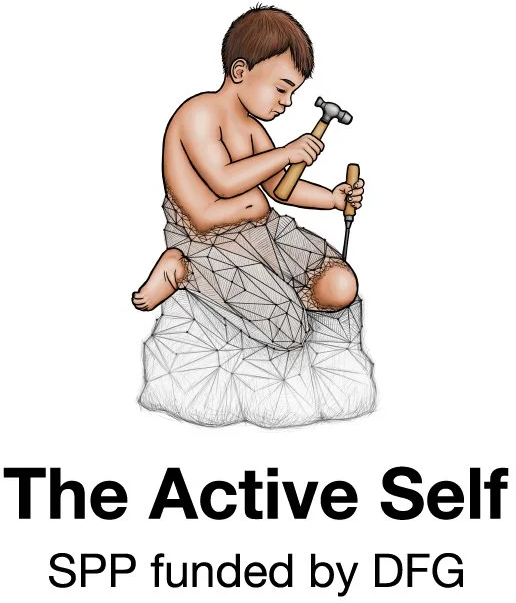
\includegraphics[height=7em]{active_self_logo_color}
		\end{minipage}
		\hfill
		\begin{minipage}[r]{0.1\textwidth}
			
\includegraphics[height=6.5em]{TUC_AI_color}
		\end{minipage}
	}

%%%%%%%%%%%%%%%%%%%%%%%%%%%%%%%%%%%%%%%%%%%%%%%%%%%%%%%%%%%%%%%%%%
% use height in headerbox to align multiple boxes 
% height= <size in percent of column height>, else [auto]%
\headerbox{The Basal Ganglia - Intralaminar Nuclei Prediction Circuit}{name=overview, column=0, row=0, span=6}{
\begin{adjustbox}{minipage=\textwidth, margin=2pt, center}

    \centering
    \begin{minipage}{0.26\textwidth}
        \textbf{Agency:}\\
        Agency, our sense of action control, relies on predicting outcomes from internal states. While the cerebellum likely plays a key role, the basal ganglia (BG) - intralaminar nuclei (ILN) circuit may also contribute. The cerebellum potentially enhances agency by generating predictive models, processing error signals, and optimizing timing of motor and cognitive processes \parencite{sendhilnathan2024cerebro}. These functions improve our ability to anticipate action results in BG-ILN loops, reinforcing our sense of agency \parencite{haggard2017sense}.\\
        
        \textbf{BG-ILN connectivity:}\\
        Various BG and ILN regions are strongly interconnected forming loops \parencite{cover_rostral_2021, gonzalo-martin_micropopulation_2024, smith_thalamostriatal_2014}. Thalamo-striatal projections are relevant for behavioral switching, attentional shifting, and reinforcement \parencite{smith_thalamostriatal_2014,cover_activation_2019, cover_rostral_2023}. Particularly the centromedian/parafascicular (CM/Pf) complex also projects to the subthalamic nucleus (STN), external globus pallidus (GPe), and internal globus pallidus/substantia nigra pars reticulata (GPi/SNr) \parencite{gonzalo-martin_micropopulation_2024,castle_thalamic_2005,kita_intralaminar_2016,hanini-daoud_processing_2022}, with branched axons that simultaneously target both the STN and the GPi/SNr. Additionally, the ILN responds to attention-related salient stimuli, suggesting its role in adapting behavior based on prediction errors \parencite{minamimoto_participation_2002,smith_thalamostriatal_2014}.
    \end{minipage}
    \hspace{0.01\textwidth}
    \begin{minipage}{0.25\textwidth}
        \centering
        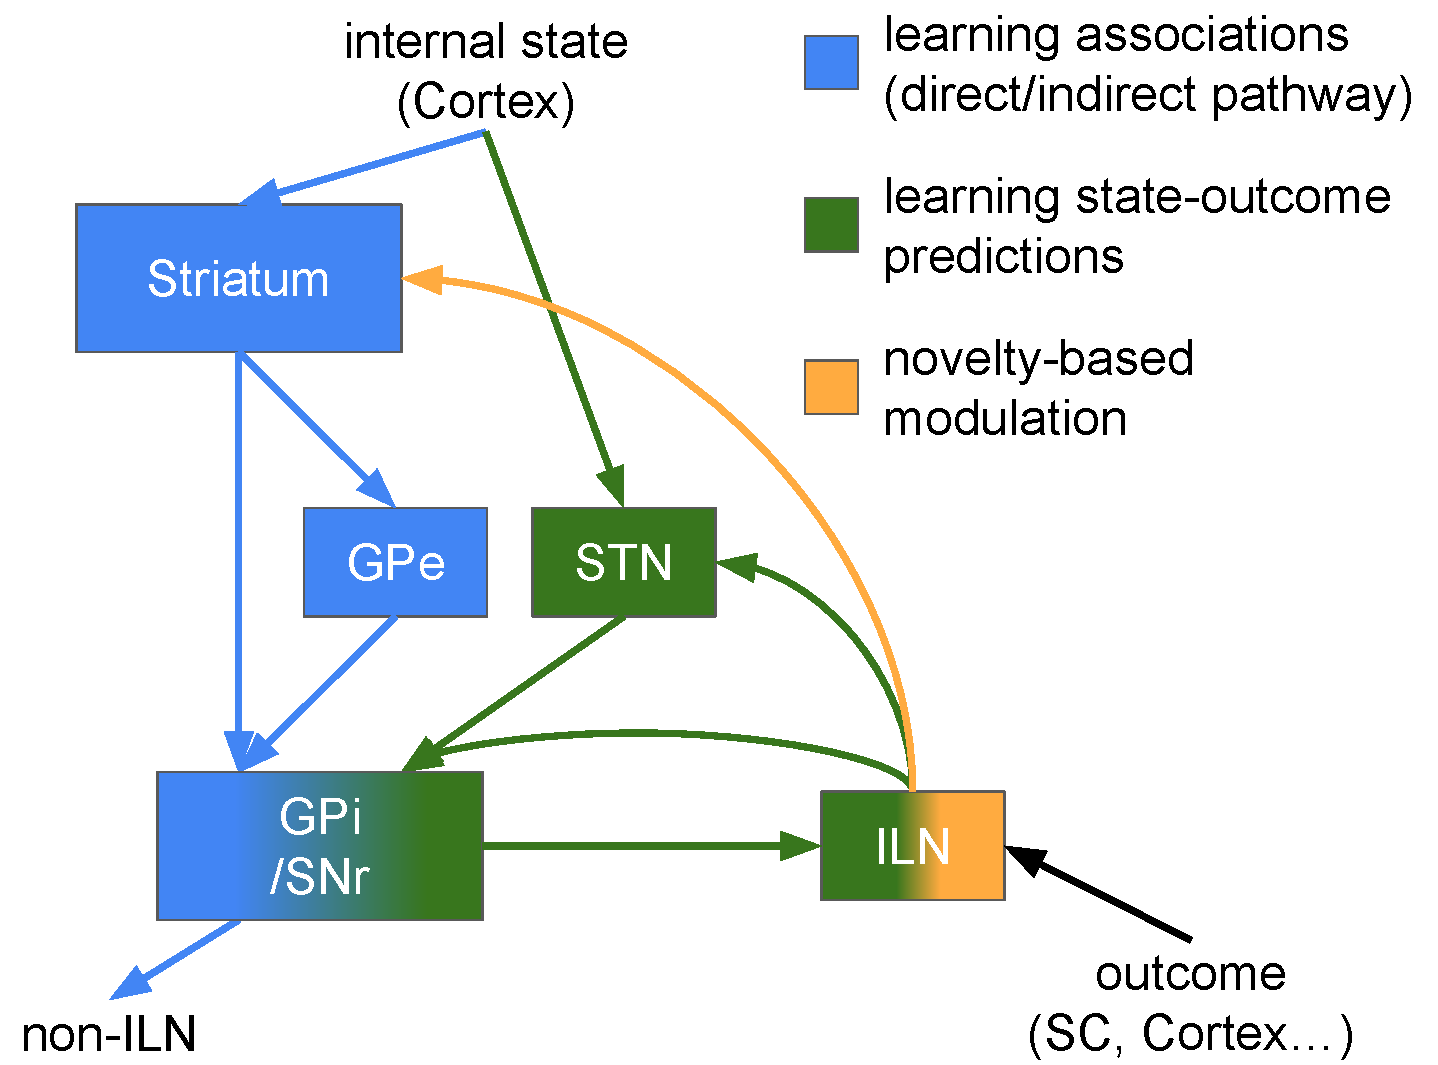
\includegraphics[width=\textwidth]{figures/circuit_idea_1.pdf}
        \textbf{Figure 1:} BG-ILN connectivity
    \end{minipage}
    \hspace{0.01\textwidth}
    \begin{minipage}{0.25\textwidth}
        \centering
        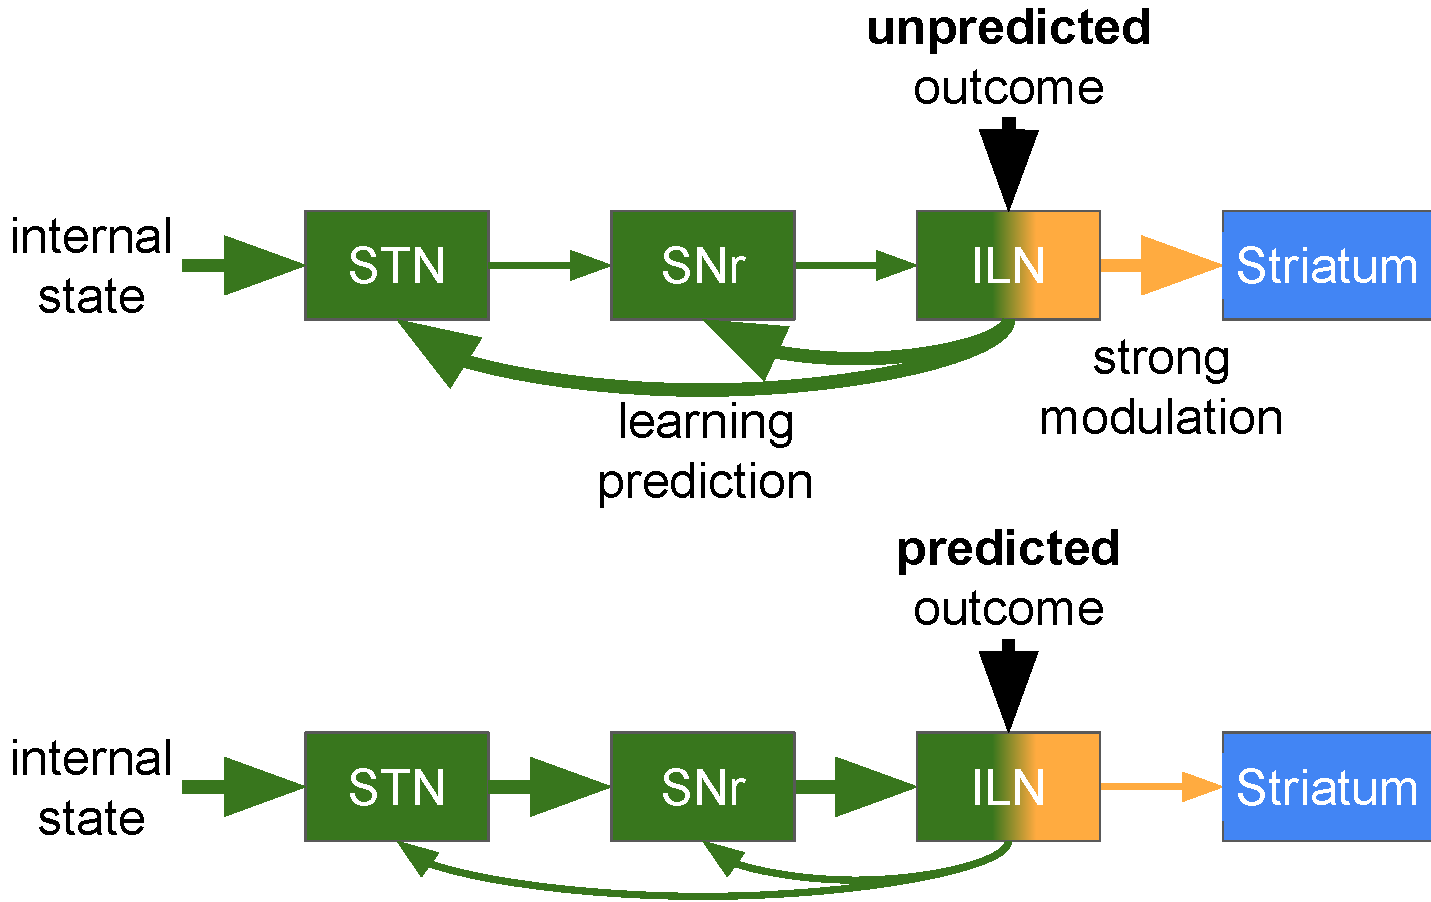
\includegraphics[width=\textwidth]{figures/circuit_idea_2.pdf}
        \textbf{Figure 2:} Prediction in the BG-ILN circuit
    \end{minipage}
    \hspace{0.01\textwidth}
    \begin{minipage}{0.18\textwidth}
        \textbf{Hypotheses:}\\
        \vfill
        \textit{Functional}
        \begin{itemize}
            \item Modulated by the branched axons from the ILN, the STN-SNr pathway learns to associate internal states with outcomes that may involve internal or external events.
            \item The prediction of an outcome is reflected in increased inhibition of the ILN by the SNr, which diminishes the ILN's response to the corresponding outcomes.
        \end{itemize}
        \vspace{5pt}
        
        \textit{General}
        \begin{itemize}
            \item The activity of the ILN represents a kind of prediction error.
            \item The BG - ILN circuits contribute to the sense of agency
            \item The BG - ILN circuits contribute to novelty detection
            \item The BG - ILN circuits contribute to information (novelty) seeking
        \end{itemize}        
    \end{minipage}
    \hfill

\end{adjustbox}
}



\headerbox{Experimental Setup}{name=exp, column=0, below=overview, span=6}{
\begin{adjustbox}{minipage=\textwidth, margin=2pt, center}
 
    \centering
	\begin{minipage}{0.26\textwidth}
		\setlist{noitemsep}
		\textbf{Experimental paradigm} \cite{minamimoto_participation_2002}:
		\begin{itemize}
			\item Hold button is illuminated $\rightarrow$ monkeys have to hold the illuminated button
            \item They have to fixate on a central LED throughout the trial
            \item After a random delay (500-1500 ms), one of two large LEDs (left or right) lights up as a cue
            \item At 100, 400, or 700 ms after the cue onset one of the two large LEDs lights up as a target
            \item If monkeys release the button within 500 ms after the target appearance they receive a reward
            \item Random intertrial interval (3-5s)\\
		\end{itemize}
        \textbf{Experimental findings:}\\
        Neurons of the CM/PF complex responded to light flashes (the cues/targets) presented on the contralateral side. However, responses to target stimuli appearing on the contralateral side depended highly on the cue condition. Neurons responded to invalidly cued targets but responded less intensely to validly cued targets.\\
	\end{minipage}
    \hspace{0.01\textwidth}
	\begin{minipage}{0.25\textwidth}
        \begin{center}
            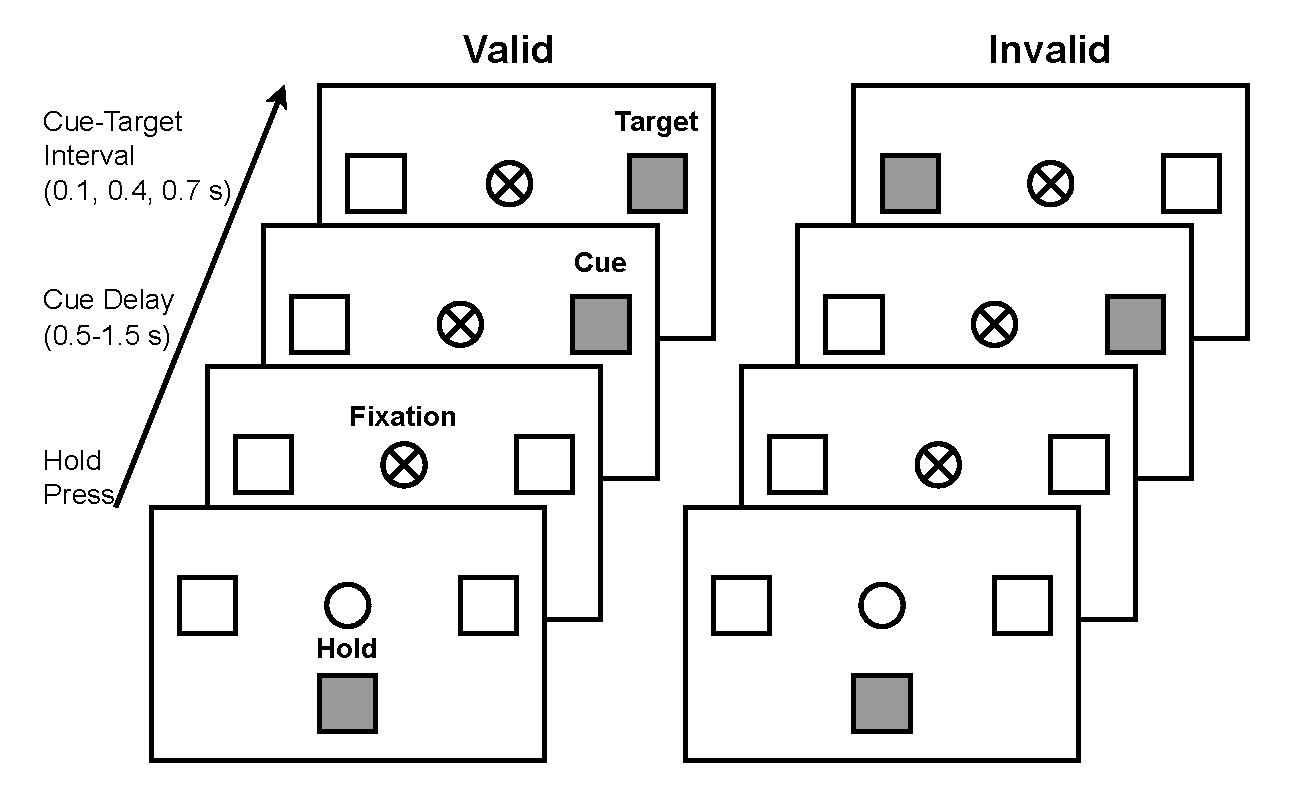
\includegraphics[width=\linewidth]{exp.pdf}
            
            \textbf{Figure 3:} Experimental paradigm. \\
            {\fontsize{4pt}{4.8pt}\selectfont (Illustration created based on Figure 1 from \parencite{minamimoto_participation_2002})} \\

            \vspace{5pt}
            
            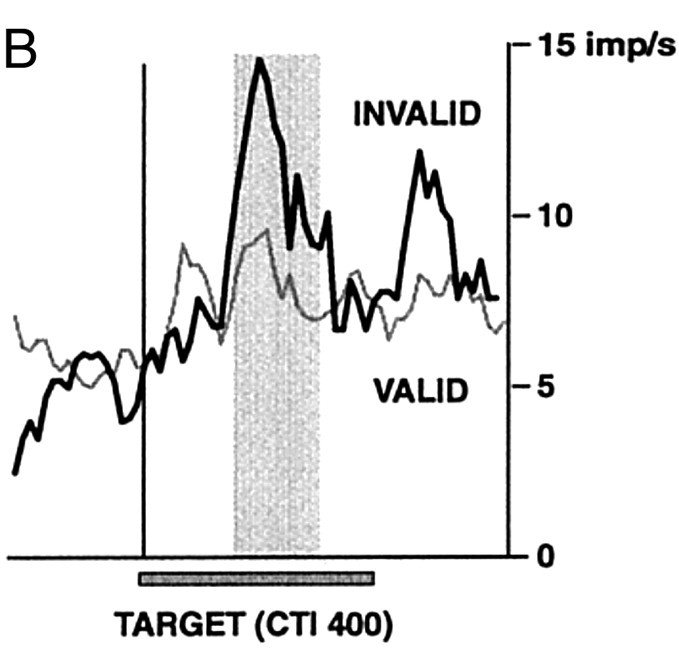
\includegraphics[width=0.5\linewidth]{exp_results.jpeg}
            
            \textbf{Figure 4:} Experimental findings. \\
            {\fontsize{4pt}{4.8pt}\selectfont (Illustration is part of Figure 5 from \parencite{minamimoto_participation_2002})} \\
        \end{center}
	\end{minipage}
    \hspace{0.01\textwidth}
	\begin{minipage}{0.25\textwidth}
        \centering
        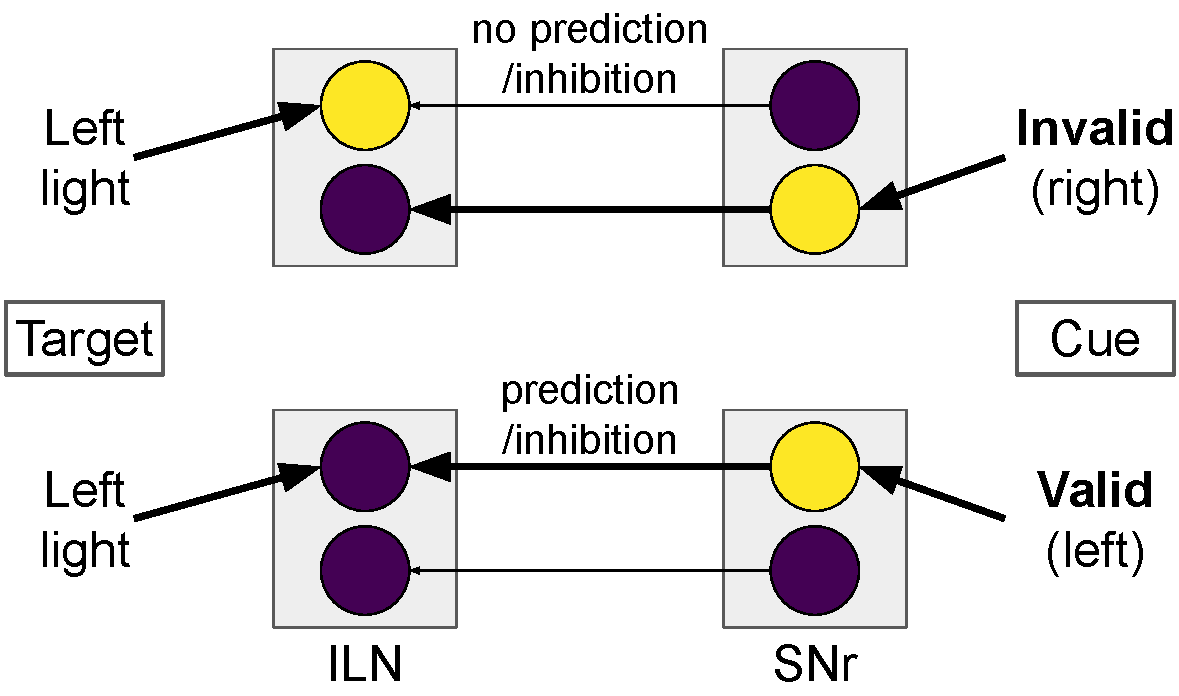
\includegraphics[width=\linewidth]{figures/exp_interpretation.pdf}
        
        \textbf{Figure 5:} Cues predict targets
	\end{minipage}
    \hspace{0.01\textwidth}
	\begin{minipage}{0.18\textwidth}        
        \textbf{Interpretation with BG-ILN prediction:}\\
        We propose that the presentation of a cue elicits an internal state, which, through task training, becomes associated with the appearance of a target on the same side via learning within the Cortex$\rightarrow$STN$\rightarrow$SNr$\rightarrow$CM/Pf pathway. Consequently, after training and following valid cues, CM/Pf neurons that would typically respond to the target on the cued side receive increased inhibitory input from the SNr, leading to a diminished response. In contrast, while invalid cues similarly elicit an internal state predicting a target on the cued side, the target appears on the opposite side, and the neurons responding to that side do not experience an increase in inhibition.
	\end{minipage}
    \hfill
	
\end{adjustbox}
}


\headerbox{Model}{name=model, column=0, below=exp, span=2}{
\begin{adjustbox}{minipage=\textwidth, margin=2pt, center}

	\begin{minipage}[t]{\textwidth}
        \begin{center}
            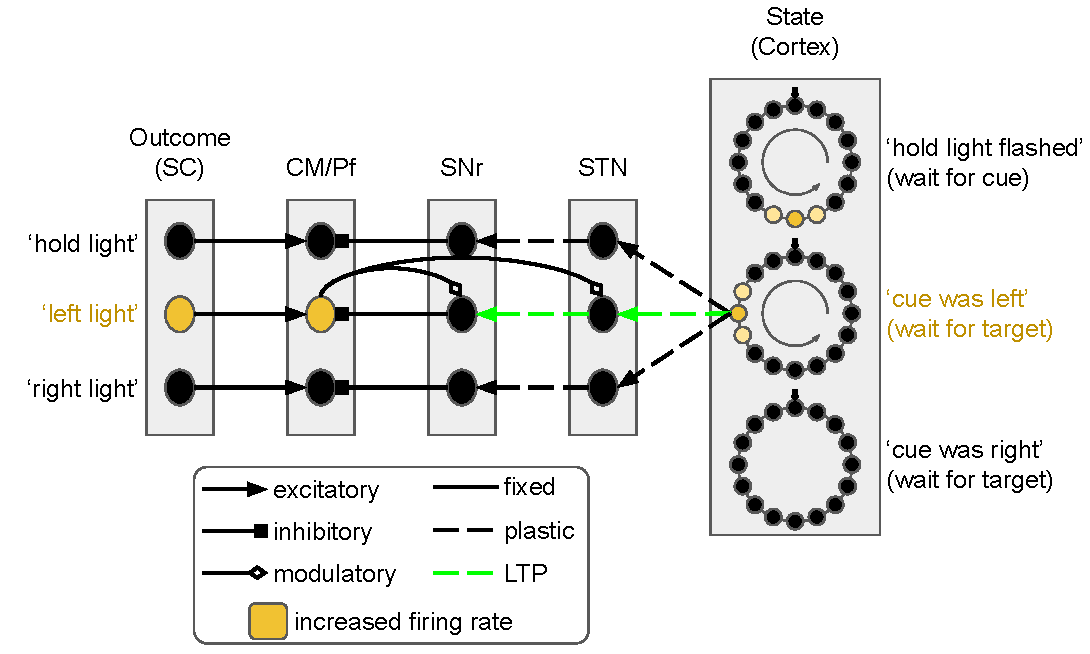
\includegraphics[width=0.8\linewidth]{model.pdf}
            
            \textbf{Figure 6:} Model overview \\
        \end{center}
        \vspace{5pt}
        - neurosimulator ANNarchy \parencite{vitay_annarchy:_2015}, rate-coded neurons \\
        - inputs to the model:
        \setlist{noitemsep}
        \begin{itemize}
            \item at hold, cue, and target light onsets: increase the firing rate of corresponding SC neurons for 50 ms
            \item after hold and cue lights: increase the firing rate of a single cortical neuron belonging to the elicited state for 200 ms (held active as response sequence)
        \end{itemize}
        - Synaptic plasticity in Cortex$\rightarrow$STN$\rightarrow$SNr:\\
        \[
        \tau \frac{dw}{dt} = \left( trace_{pre} > 0.8 \right)  \left( \text{sign(} r_{pf} - base_{pf} \text{)} - \alpha \right) \left( 1-r_{post} \right)
        \]
	\end{minipage}
		
\end{adjustbox}
}

\headerbox{References}{name=refs, column=0, below=model, above=bottom, span=5}{
    \compressbib{\printbibliography[heading=none]}
}

\headerbox{Modeling Results}{name=results, column=2, below=exp, above=refs, span=4}{
\begin{adjustbox}{minipage=\textwidth, margin=2pt, center}

    \centering
	\begin{minipage}{0.26\textwidth}
		\centering
        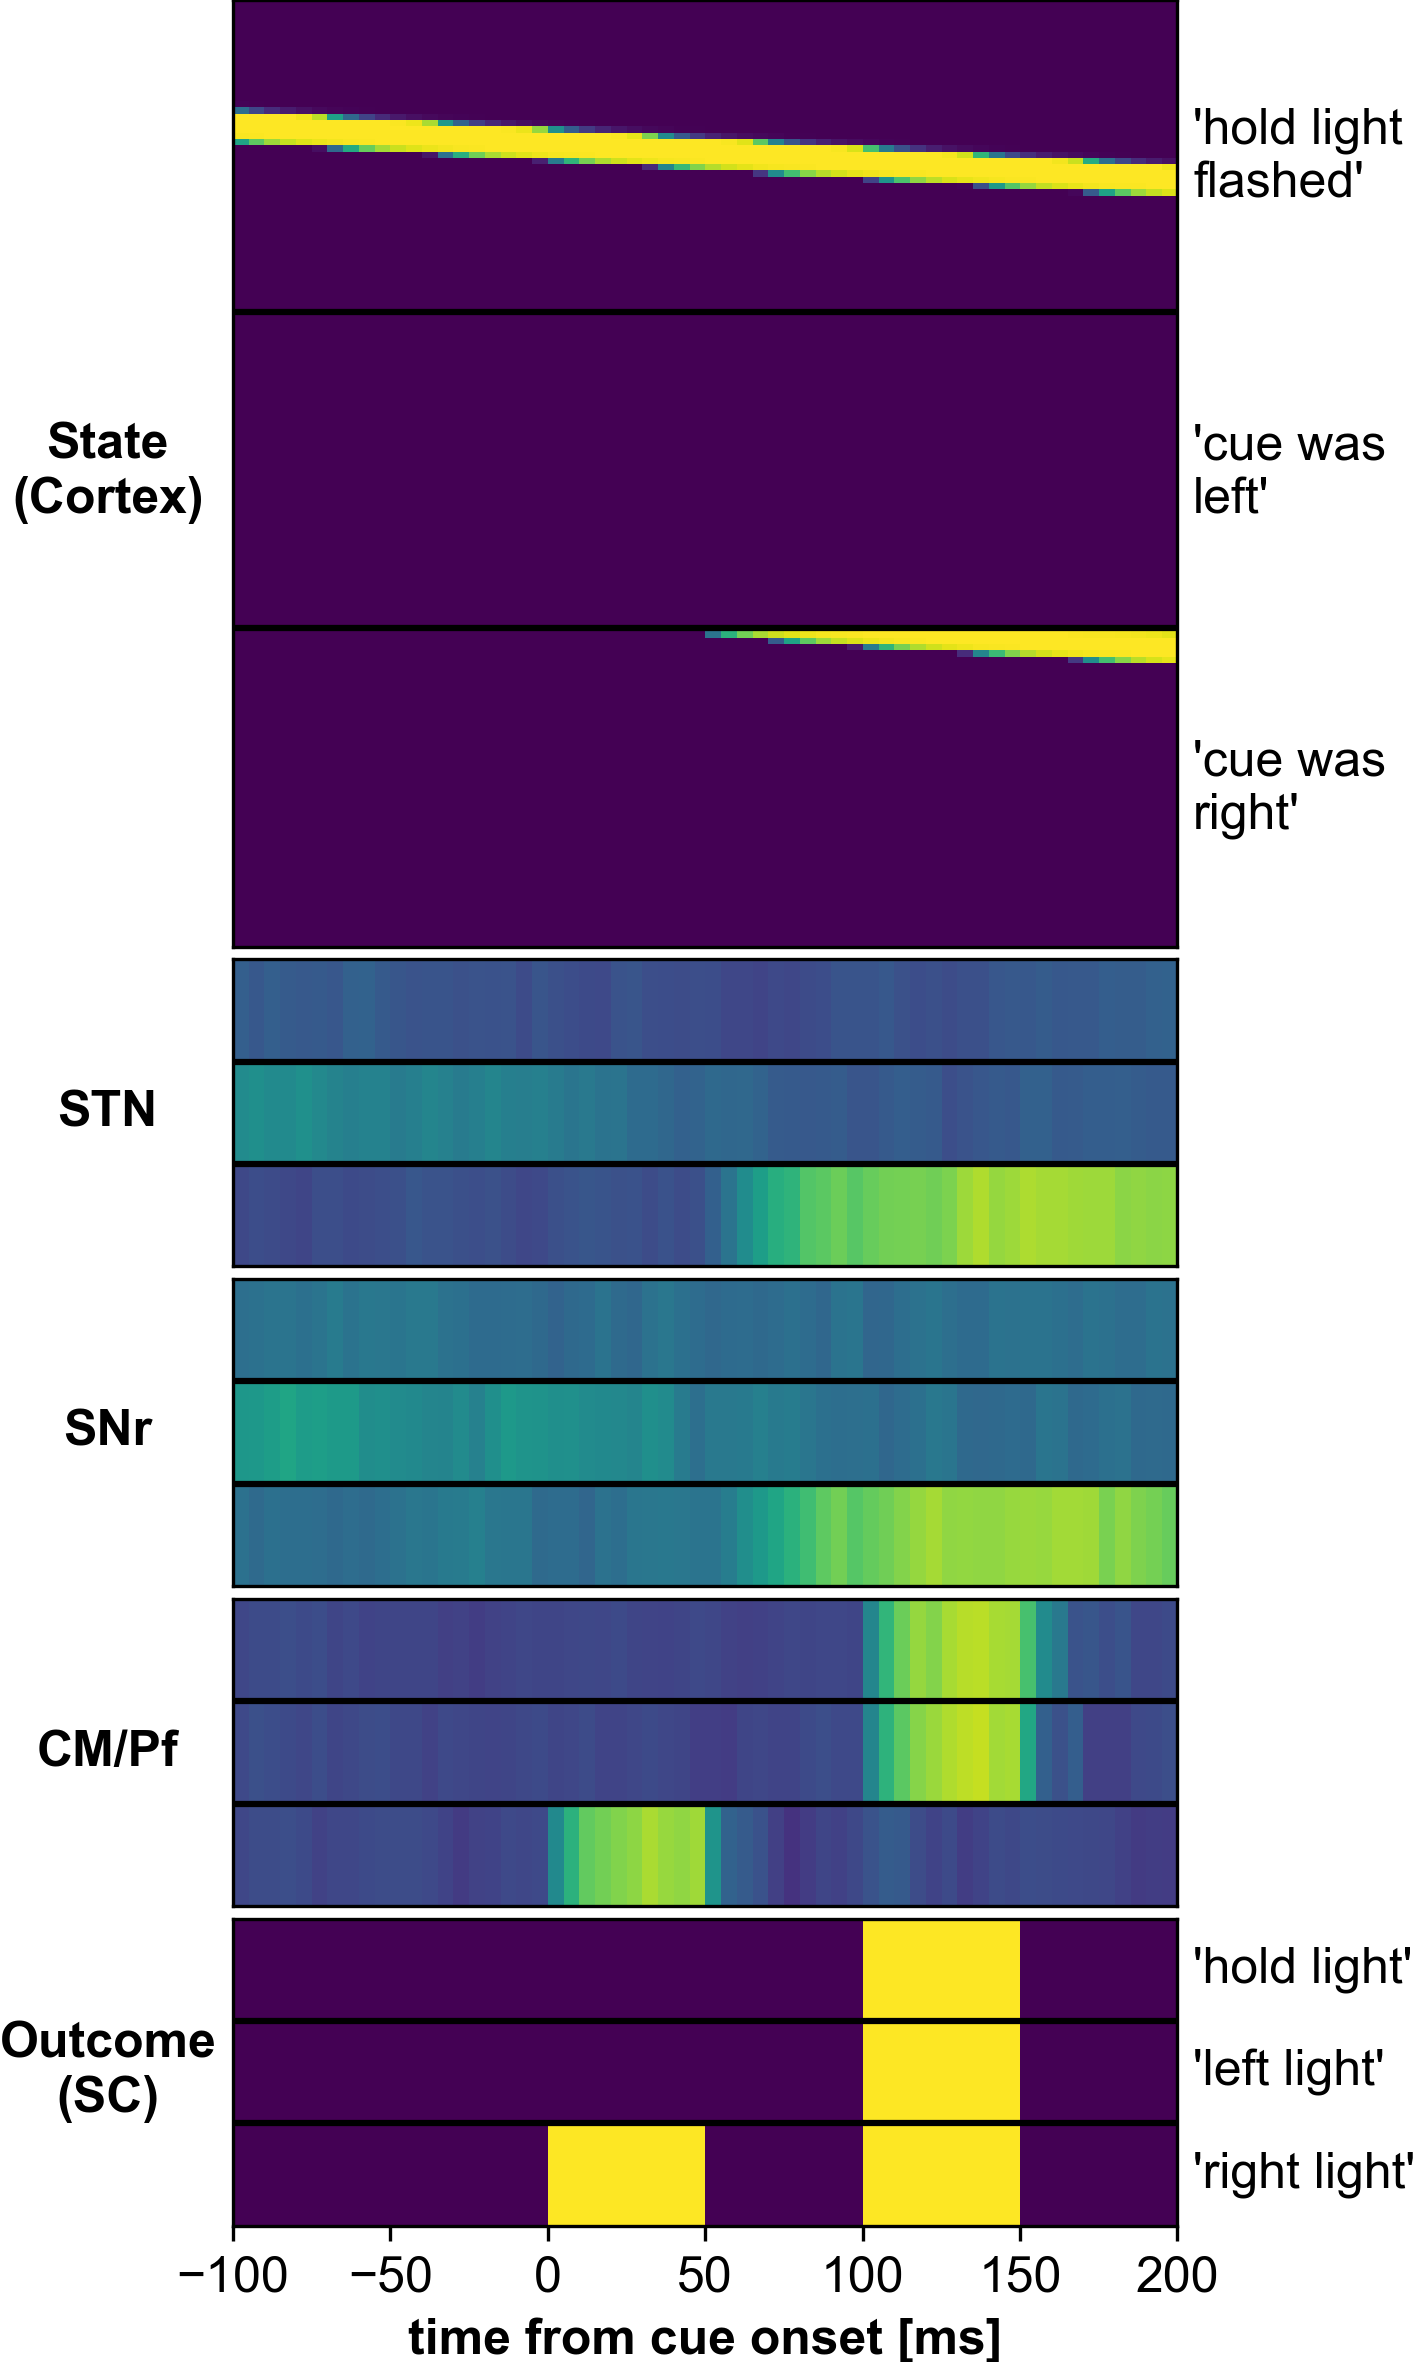
\includegraphics[width=\linewidth]{figures/single_trial_rates_cor_and_responses_matrix.png}
        
        \textbf{Figure 7:} Firing rates single trial
	\end{minipage}
    \hspace{0.01\textwidth}
	\begin{minipage}{0.18\textwidth}
        Firing rates of the model’s neurons during the cue and target presentation (cue-target interval = 100 ms) in a single trial after learning are shown. At target onset, all three outcomes are activated in this trial. The cue ‘right light’ elicits the state 'cue was right' in the cortex, and in the STN and SNr, neurons associated with the outcome 'right light' exhibit increased firing rates. This illustrates the learned association 'cue was right' $\rightarrow$ 'right light'. The Pf responds to excitatory input from the SC, but only when the inhibitory input from the SNr is not increased.
	\end{minipage}
    \hspace{0.05\textwidth}
	\begin{minipage}{0.48\textwidth}  
        \begin{center}
            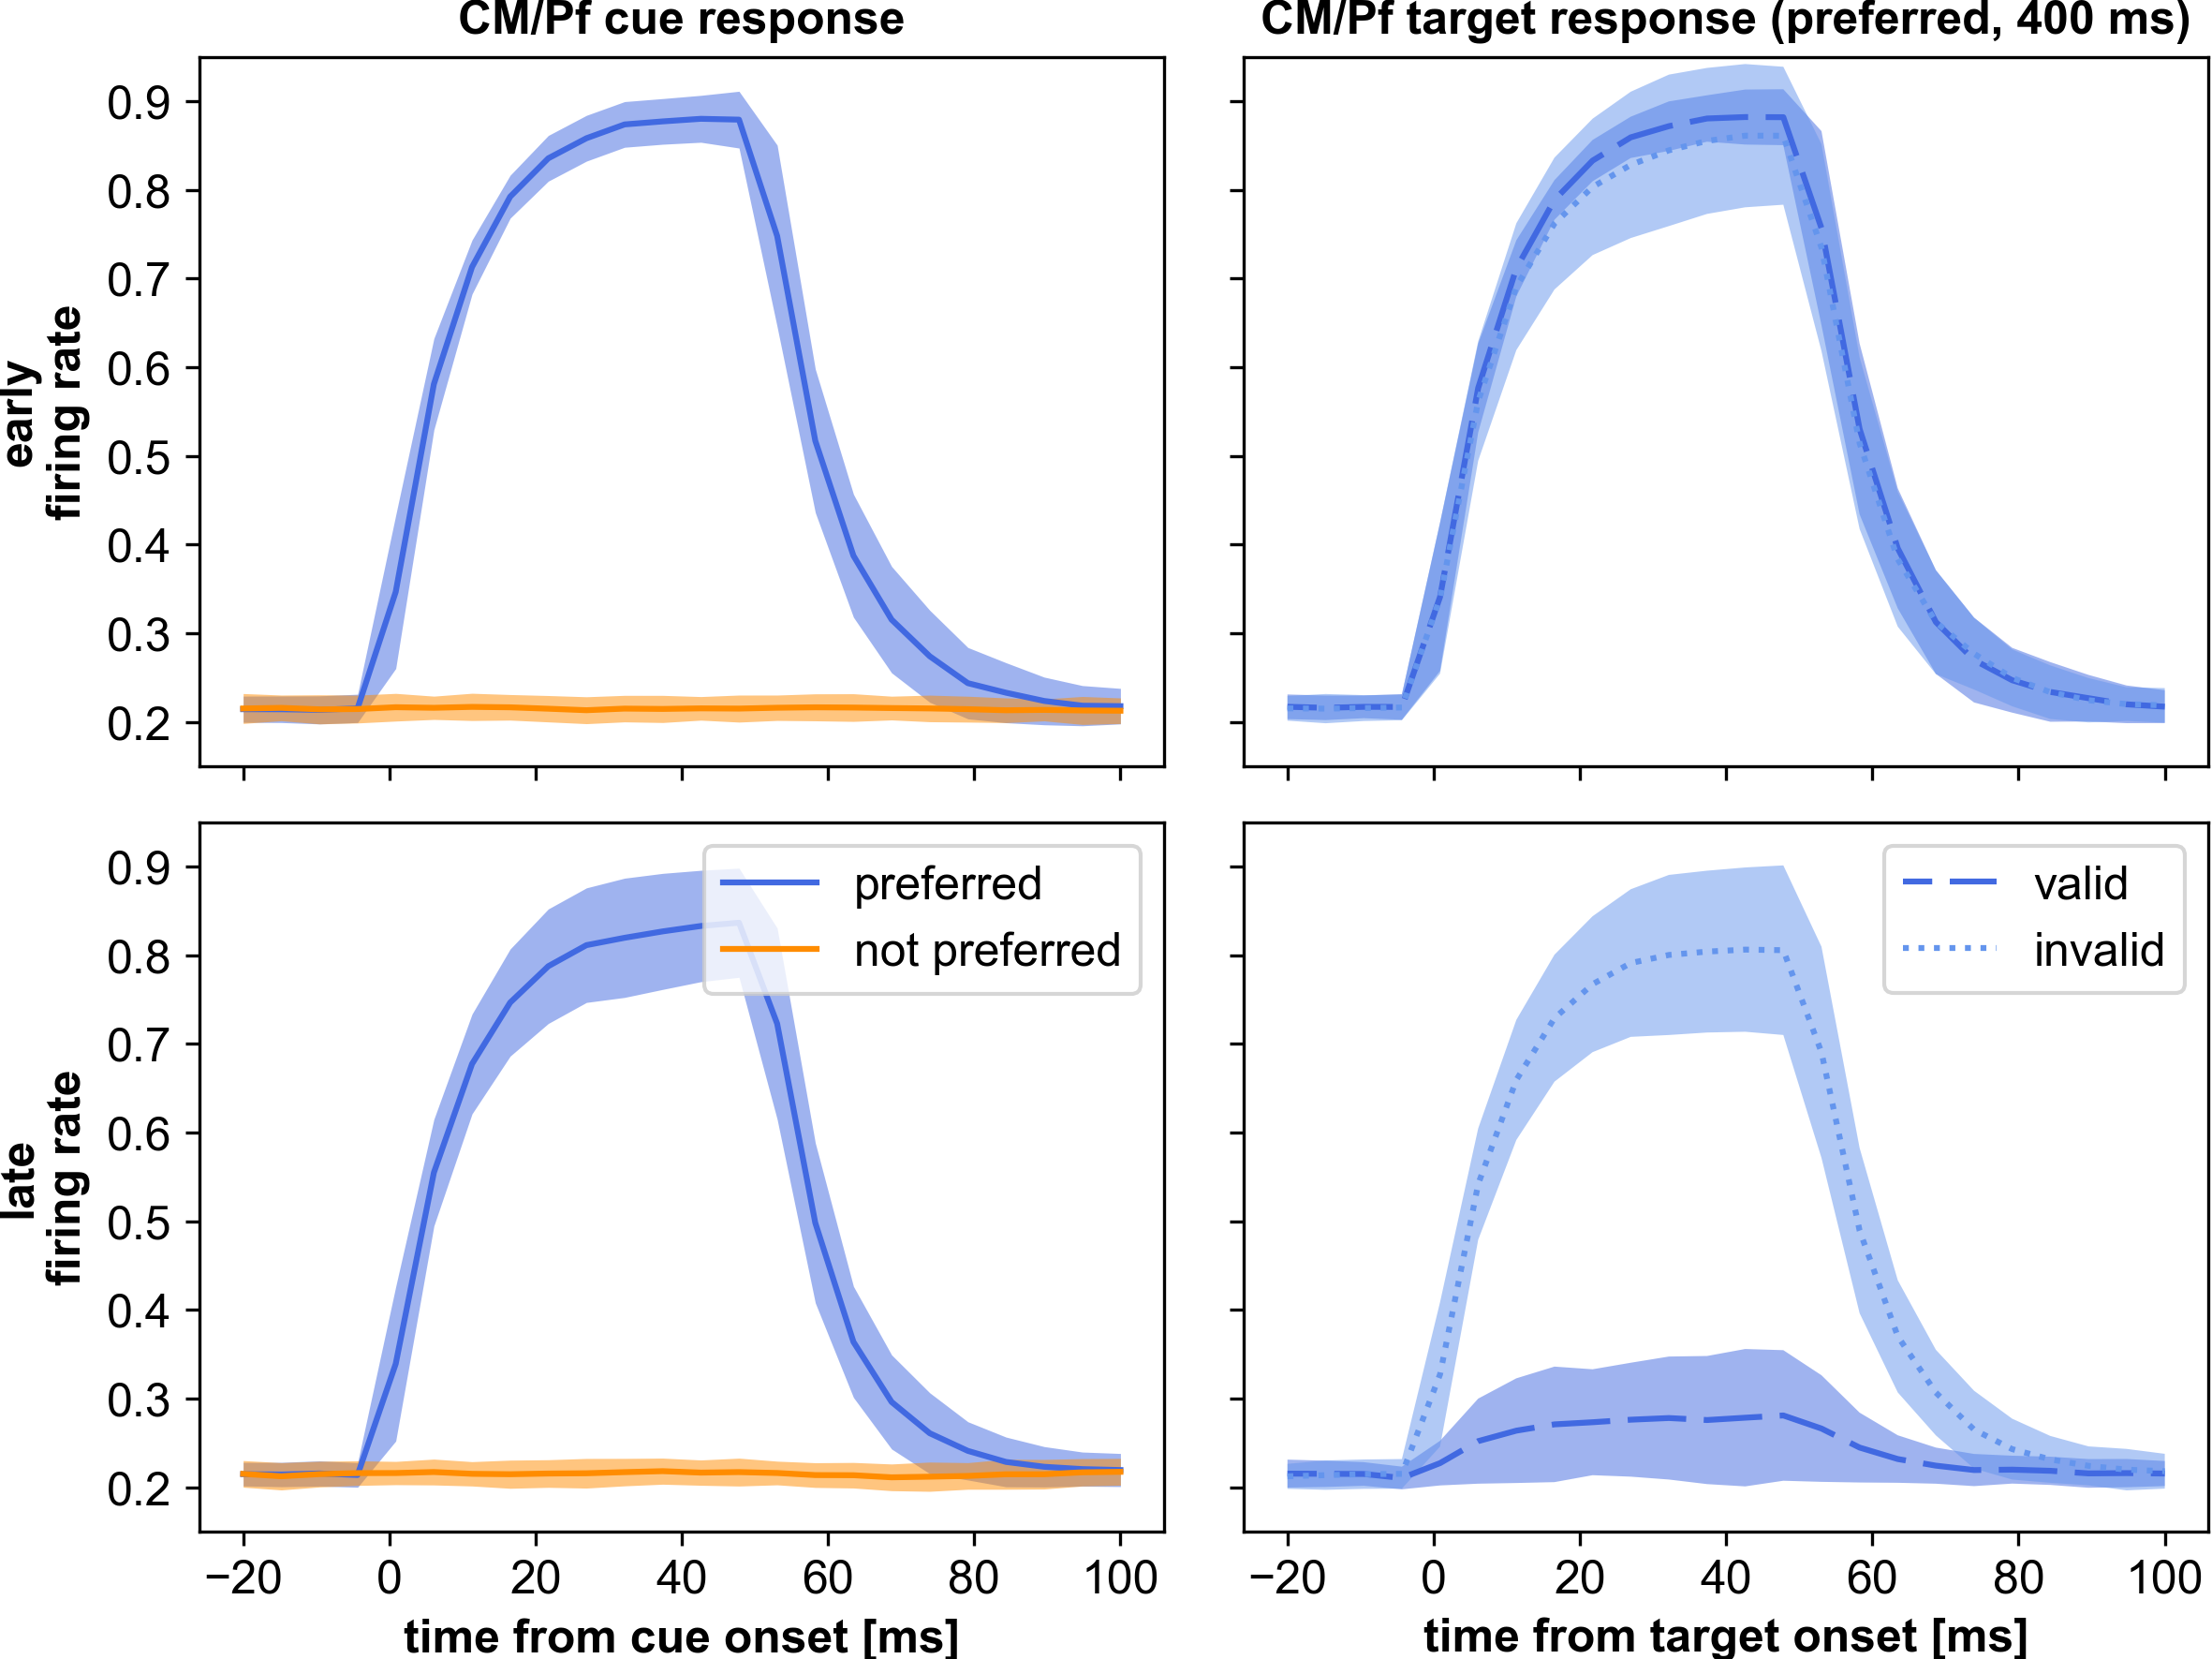
\includegraphics[width=0.75\linewidth]{figures/pf_response.png}
            
            \textbf{Figure 8:} Firing rates single trial \\
        \end{center}
        \vspace{5pt}
        Responses of Pf neurons to cues and targets averaged over the first and last 100 trials (before and after training) of each respective category. The response to the cues does not change significantly after training. In contrast, the response to the targets depends on the cue validity after task training. The response to invalidly cued targets does not change but the response to validly cued targets decreases as in \parencite{minamimoto_participation_2002}.
	\end{minipage}
    \hfill
  
\end{adjustbox}
}



\headerbox{\normalsize Acknowledgements}{name=ack, column=5, below=model, above=bottom, span=1}{
\begin{adjustbox}{minipage=\textwidth, margin=2pt, center}

    \centering
	\begin{minipage}{\textwidth}
		This work was supported by the DFG priority program ”The Active Self” HA2630/12-2.\\[5pt]
	\end{minipage}
	\begin{minipage}{\textwidth}
	\begin{center}
        
\includegraphics[width=0.8\linewidth]{qr-code}
	\end{center}
	\end{minipage}
    \hfill
 
\end{adjustbox}
}





\end{poster}


\end{document}